\documentclass[border=4pt]{standalone}

% --- packages (mirror these in network.meta.json "requires") ---
\usepackage{tikz}

% --- palette (canonical source: reference/color-palettes/color-palettes.md; light variant) ---
\definecolor{otblue}{HTML}{0072B2}
\definecolor{otorange}{HTML}{E69F00}
\definecolor{otteal}{HTML}{009E73}
\definecolor{otpurple}{HTML}{CC79A7}
\definecolor{otgray}{HTML}{5A5A5A}

\begin{document}
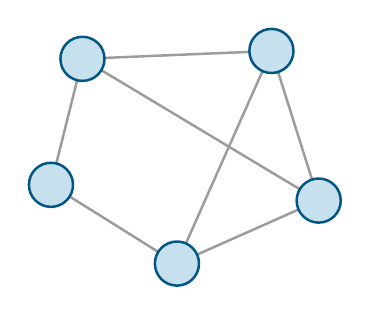
\begin{tikzpicture}[line width=0.9pt]
  % node positions: an interconnected mesh of peers
  \coordinate (a) at (0.0,1.4);
  \coordinate (b) at (2.4,1.5);
  \coordinate (c) at (3.0,-0.4);
  \coordinate (d) at (1.2,-1.2);
  \coordinate (e) at (-0.4,-0.2);
  % links (outer ring + two cross-links)
  \foreach \p/\q in {a/b,b/c,c/d,d/e,e/a,a/c,b/d}{ \draw[otgray!60] (\p) -- (\q); }
  % nodes
  \foreach \n in {a,b,c,d,e}{
    \filldraw[draw=otblue!75!black, fill=otblue!22] (\n) circle[radius=0.28];
  }
\end{tikzpicture}
\end{document}
